\documentclass{ctexart}

\usepackage{listings}

\title{FPGA 作业 (II)}
\author{李约瀚 \\ 14130140331 \\ qinka@live.com \\ qinka@qinka.pw}

\lstset{breaklines}

\begin{document}

% Cover
\thispagestyle{empty}
\begin{center}
  \vspace*{4em}
  {\Huge\textbf{FPGA 作业 \\ \vspace*{0.5em} (II)}}
  \vfill
  \large
  \begin{tabular}{c@{:}l}
    班级 & 14113014 \\
    学号 & 14130140331 \\
    姓名 & 李约瀚 \\
    教师 & 沈沛意 \\
  \end{tabular}
  \vspace*{4em}\\
\end{center}
\newpage

\section{层次化工程创建}

\subsection{实验目的}
\begin{itemize}
\item 熟悉简单逻辑门的RTL描述
\item 创建简单电路的结构化描述
\item 用 VHDL 创建层次结构描述
\item 熟悉 ISE 集成环境中的 HDL 编辑器
\end{itemize}


\subsection{实验步骤}

\begin{enumerate}
\item 使用 ISE 创建新的工程
\item 完成逻辑门的 RTL 描述
\item 检查代码中的语法错误并生成原理图
\end{enumerate}


\subsection{报告正文}

\subsubsection{创建一个新工程}

打开 \verb|Xilinx ISE| 在文件中选择创建新的工程项目,并配置相对应的路径。
点击下一步,然后配置与 Spartan-6 和开发版 Nexys3 有关的配置,然后并继续配置。

\subsubsection{逻辑门的 RTL 描述}

在工程中选择新建源码,并将其命名为 \verb|MY_AND2.vhd|。然后为其输入代码:
\begin{lstlisting}[language=VHDL]
library IEEE;
use IEEE.STD_LOGIC_1164.ALL;

entity my_and2 is
    Port ( A : in  STD_LOGIC;
           B : in  STD_LOGIC;
           C : out  STD_LOGIC);
end my_and2;

architecture Behavioral of my_and2 is
begin
	C <= A and B;
end Behavioral;
\end{lstlisting}

并通过同样的方式创建文件 \verb|MY_OR2.vhd|。然后输入代码:
\begin{lstlisting}[language=VHDL]
library IEEE;
use IEEE.STD_LOGIC_1164.ALL;

entity my_or2 is
    Port ( A : in  STD_LOGIC;
           B : in  STD_LOGIC;
           C : out  STD_LOGIC);
end my_or2;

architecture Behavioral of my_or2 is
begin
	C <= A or B;
end Behavioral;
\end{lstlisting}

然后是文件 \verb|AND_OR.vhd|。并输入代码:
\begin{lstlisting}[language=VHDL]
library IEEE;
use IEEE.STD_LOGIC_1164.ALL;

entity and_or is
  Port ( INP: in STD_LOGIC_VECTOR(3 downto 0);
           Z: out STD_LOGIC);
end and_or;

architecture Struct of and_or is
  component my_and2
    port( A: in  STD_LOGIC;
          B: in  STD_LOGIC;
          C: out STD_LOGIC);
  end component;
  component my_or2
    port( A: in  STD_LOGIC;
          B: in  STD_LOGIC;
          C: out STD_LOGIC);
  end component;

signal s1,s2:STD_LOGIC;
begin
  U0: my_and2 port map (A => INP(0), B => INP(1), C => s1);
  U1: my_and2 port map (A => INP(2), B => INP(3), C => s2);
  U2: my_or2  port map (A => S1    , B => S2    , C => Z );
end struct;
\end{lstlisting}

\subsubsection{语法检查并生成原理图}

在 ISE 中选中顶层模块 AND\_OR,在 Proccess 中进行综合,在 Synthesize 中双击 
\verb|Check Syntax| 检查语法。并修正有错误的语法。
然后在选中 \verb|View RTL Schematic| 生成并查看原理图,如图 \ref{fig:homework2-3}。

\begin{figure}
\centering
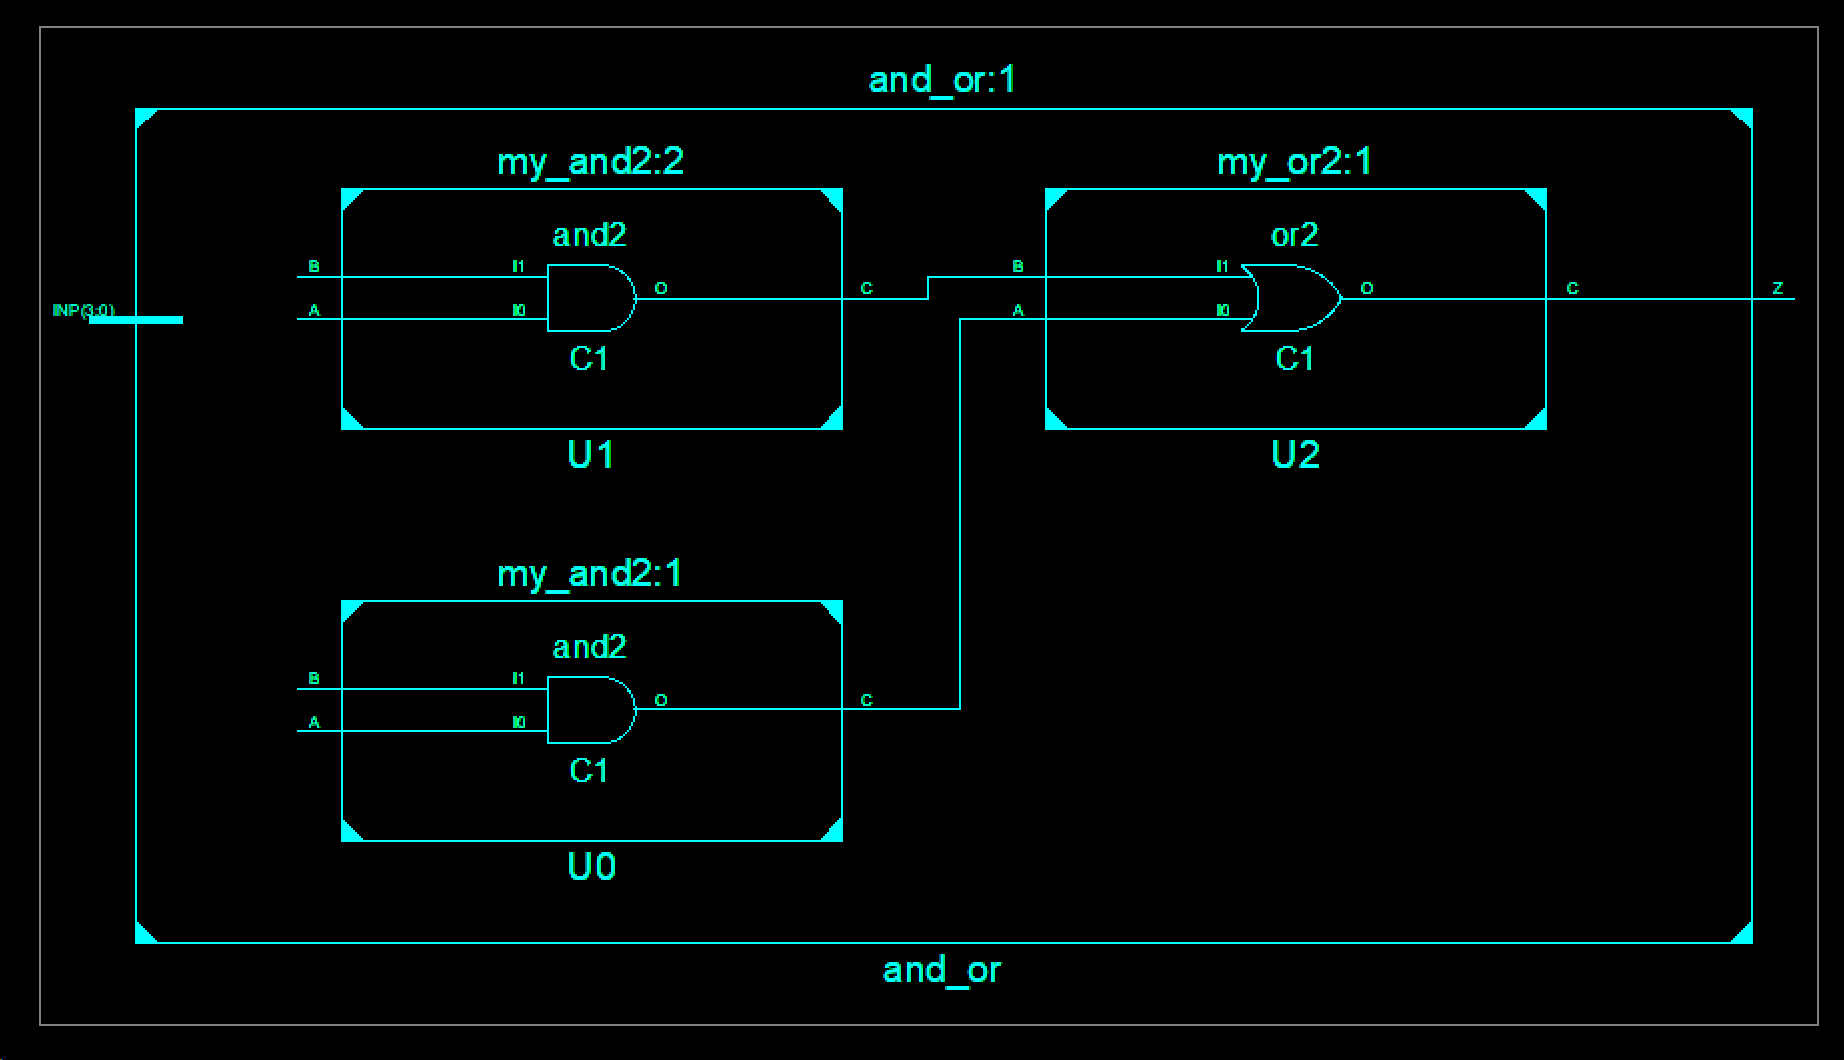
\includegraphics[width=1\linewidth]{homework2-3}
\caption{原理图}
\label{fig:homework2-3}
\end{figure}



\subsection{额外步骤}

在配置检查原理图之后,为项目添加 约束文件,代码如下:
\begin{lstlisting}
NET "INP[0]" LOC = T10;
NET "INP[1]" LOC = T9;
NET "INP[2]" LOC = V9;
NET "INP[3]" LOC = M8;
NET "Z" LOC = U16;

NET "INP[3]" IOSTANDARD = LVCMOS33;
NET "INP[2]" IOSTANDARD = LVCMOS33;
NET "INP[1]" IOSTANDARD = LVCMOS33;
NET "INP[0]" IOSTANDARD = LVCMOS33;
NET "Z" IOSTANDARD = LVCMOS33;
\end{lstlisting}

将输入与波动开关绑定,然后输出绑定到LED灯。
然后进行综合生成比特流文件,并配置到开发板上。拨动开关,然后观察结果。

\section{仿真测试平台的创建}


\subsection{实验目的}
\begin{itemize}
    \item 创建一个测试平台文件,测试实验一中的 AND\_OR 模块。验证其正确性
    \item 学习 ISE 中测试平台向导
    \item 建立基本的输入激励
    \item 学习仿真验证方法
\end{itemize}


\subsection{实验步骤}

\begin{enumerate}
    \item 使用 ISE 创建新的工程
    \item 创建一个测试平台文件
    \item 创建简单的输入激励
    \item 验证 AND\_OR 逻辑结构
\end{enumerate}


\subsection{报告正文}

\subsubsection{创建一个新工程}

打开 \verb|Xilinx ISE| 在文件中选择创建新的工程项目,并配置相对应的路径。
点击下一步,然后配置与 Spartan-6 和开发版 Nexys3 有关的配置,然后并继续配置。

并将之前实验的内容中的代码导入现在的工程中。

\subsubsection{创建一个简单测试平台平台文件}

使用测试平台向导创建一个测试平台文件。
在项目工程中选择新添加源代码,然后选择 VHDL Test Bench 作为源文件类型,然后然后为其添加名字。
并将顶层模块与之关联。

自动创建好的内容有:
\begin{itemize}
    \item 被测试的顶层元件声明
    \item 顶层信号声明
    \item 元件实例化与端口映射
    \item 测试激励输入的外部描述结构
\end{itemize}

\subsubsection{创建简单的输入激励}

我们需要对总线 INP 的信号源提供单独的激励输入。需要在 \lstinline[language=VHDL]|ARCHITECTURE| 中定义
两个信号:
\begin{lstlisting}[language=VHDL]
signal A_STIM,B_STIM : STD_LOGIC_VECTOR(1 downto 0);
\end{lstlisting}

然后在起之后的 \lstinline[language=VHDL]|BEGIN| 插入如下代码
\begin{lstlisting}[language=VHDL]
INP <= A_STIM & B_STIM : STD_LOGIC_VERCTOR (1 download 0);
\end{lstlisting}

全部代码如下所示
\begin{lstlisting}[language=VHDL]
LIBRARY ieee;
USE ieee.std_logic_1164.ALL;

ENTITY and_or_test_bench IS
END and_or_test_bench;

ARCHITECTURE test OF and_or_test_bench IS 
    COMPONENT and_or
        PORT(
            INP : IN  std_logic_vector(3 downto 0);
              Z : OUT std_logic
        );
    END COMPONENT;

    signal INP : std_logic_vector(3 downto 0); -- := (others => '0');
    signal   Z : std_logic;
    signal a_stim, b_stim: STD_LOGIC_VECTOR(1 downto 0);

BEGIN
    INP <= a_stim & b_stim;
    uut: and_or PORT MAP (
        INP => INP,
          Z => Z
        );
    a_stim <= "00","01" after 50ns, "10" after 100 ns, "11" after 150ns;

    test_bench: process
        begin
            b_stim <= "11";
            wait for 50 ns;
            b_stim <= "10";
            wait for 50 ns;
            b_stim <= "01";
            wait for 50 ns;
            b_stim <= "00";
            wait; -- !! for ever
        end process;
END test;

\end{lstlisting}

\subsubsection{验证 AND\_OR 逻辑结构}

在Sources 窗口中选择 仿真,然后先后运行语法检查与仿真两个任务。

在原型仿真之后,会出现 Xilinx 的仿真软件,同时带有着仿真结果,其结果如图 \ref{fig:homework2-2}。
一切完整后会出现会后的仿真结构,通过缩放来检查最后仿真的结构。符合元件的设计。

\begin{figure}
\centering
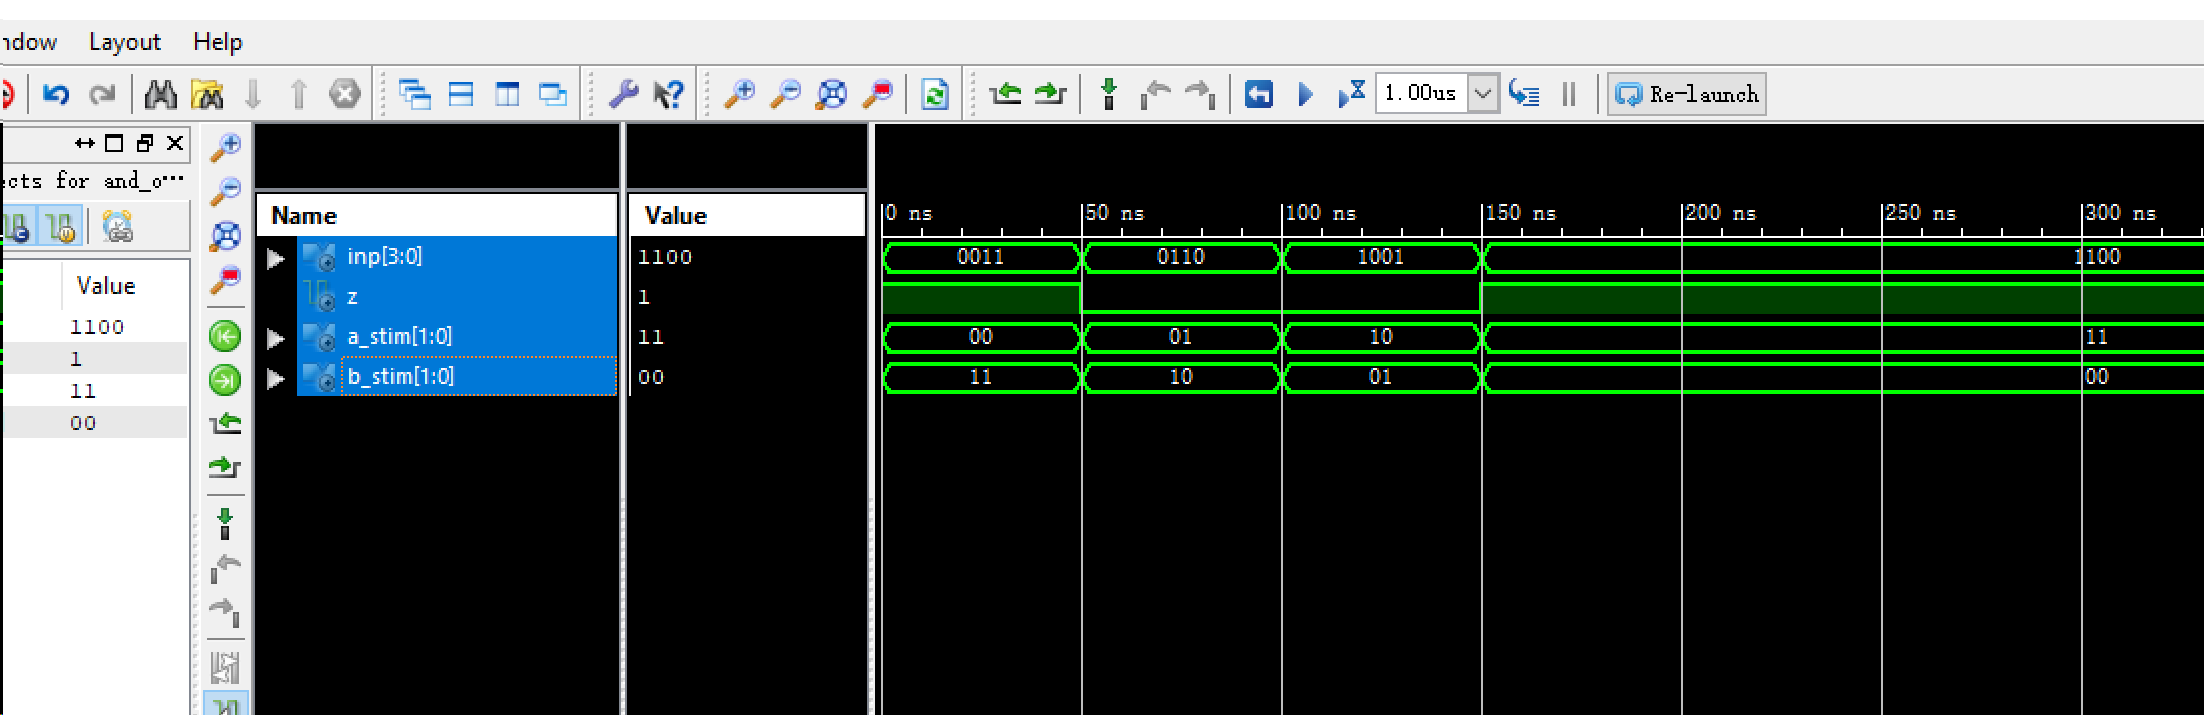
\includegraphics[width=0.7\linewidth]{homework2-2}
\caption{仿真结构}
\label{fig:report3-5}
\end{figure}



\section{熟悉 Xilinx 开发工具}

\subsection{实验目的}

\begin{itemize}
    \item 了解 FGPA 的开发流程
    \item 熟悉 Spartan-6 开发套件的功能特点
    \item 清楚 PicoBlaze 8位控制器的特性
\end{itemize}

\subsection{实验步骤}

\begin{enumerate}
    \item 启动 ISE 创建新工程
    \item 添加硬件描述代码
    \item 编译设计
    \item 仿真设计
    \item 实现设计
\end{enumerate}

\subsection{报告正文}

\subsubsection{启动 ISE 创建新工程}

打开 \verb|Xilinx ISE| 在文件中选择创建新的工程项目,并配置相对应的路径。
点击下一步,然后配置与 Spartan-6 和开发版 Nexys3 有关的配置,然后并继续配置。

\subsubsection{添加硬件描述代码}

添加官方提供的 \verb|kcpsm3.v| 与 \verb|kcpsm3_int_test.v|。
然后对于还缺少的 int\_test 模块则需要通过一定方式添加。

\subsubsection{编译设计}

在 KCPSM3 中的 Assembler 文件加中找到 kcpsm3.exe,然后在终端中运行 \lstinline|.\kcpsm3 int_test.psm|

然后会生成 int\_test 模块的文件,这里将int\_test.v 添加到了工程中。

\subsubsection{仿真设计}

添加 官方提供的仿真设计文件 \verb|testbench.v| 到工程中。 然后在 ISE 中先检查语法内容然后,执行仿真。
在执行仿真之前,设置之定义的仿真时长,这里设置为 $25000ns$。

然后Xilinx 的仿真软件的界面会出现,并且显示仿真结果,如图 \ref{fig:homework2-1}所示。

\begin{figure}
\centering
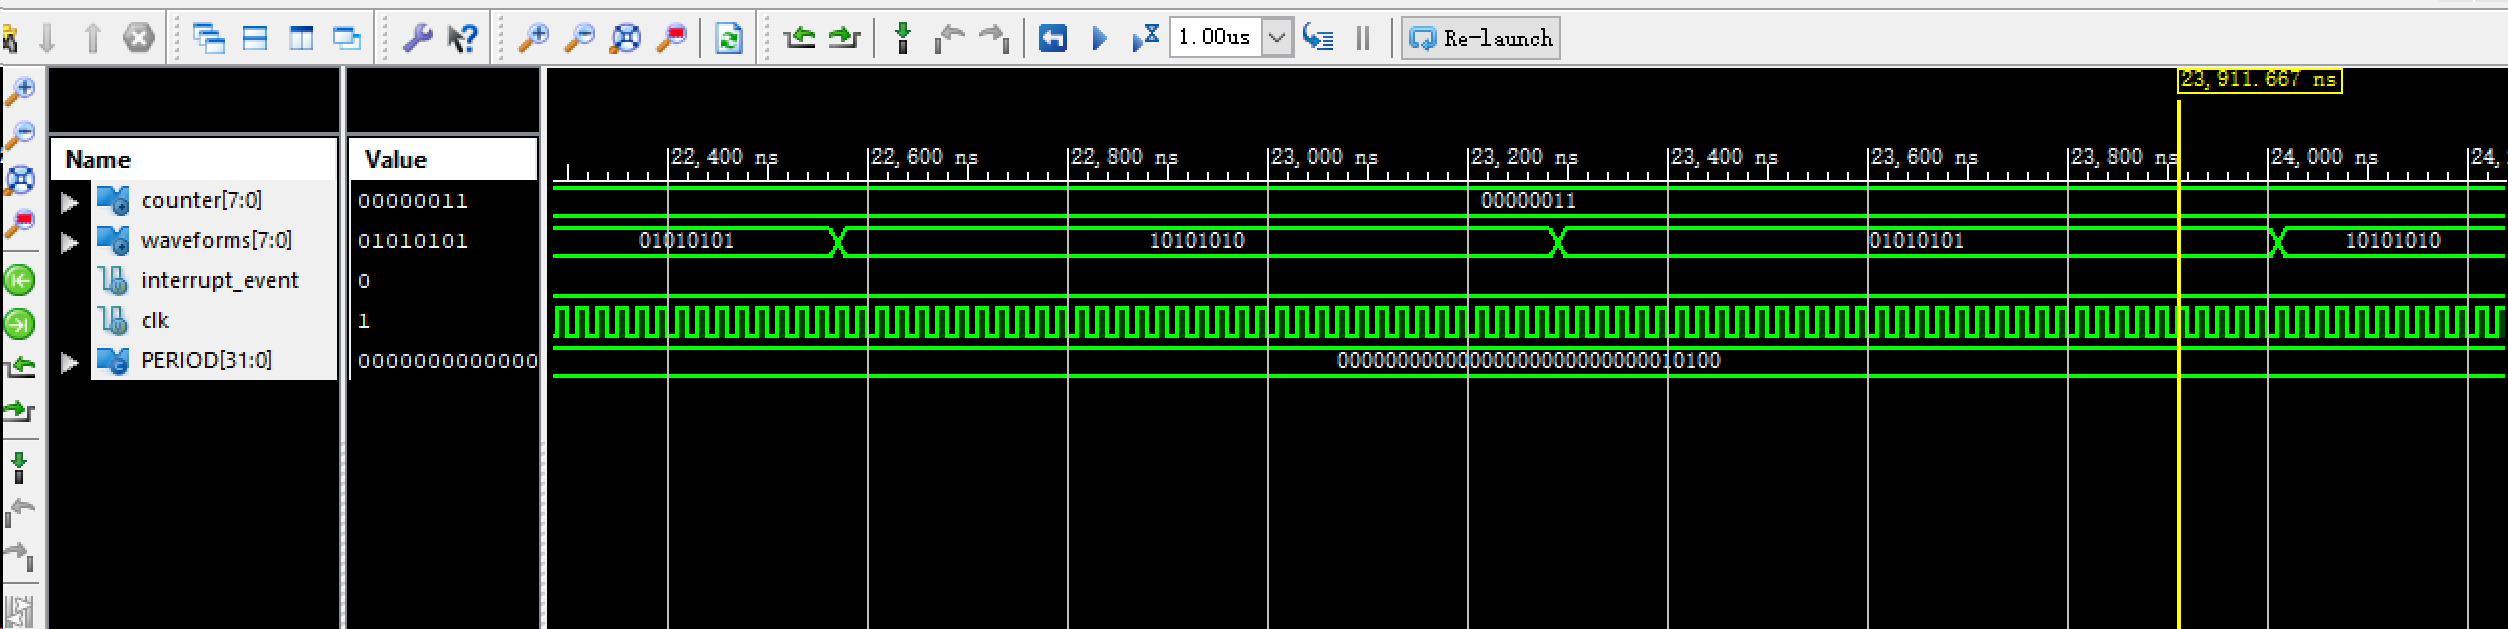
\includegraphics[width=0.7\linewidth]{homework2-1}
\caption{仿真结果}
\label{fig:report3-4}
\end{figure}


\subsubsection{设计实现}

切换回综合实现的面板,然后一次执行 Synthesize -XST 与 Implement Design 完成综合实现。

        \section{心得}
        整个实验中,使用的开发版与 ISE 的版本与书中的版本相差较大,但是打他相对还是可以完成。其中对于第三个实验中使用的 kcpsm3 在当前的 Windows 10 慢速更新预览版上无法使用且与 开发版不兼容问题,我尝试将 kcpsm6 按照实验要求完成。虽然总线位数不是问题,但是由于对系统不熟悉,最后移植的结果并不能让人满意,仿真无输出结果。最后只能通过其他方式进行实验,并仿真。

\end{document}